\documentclass{article}
\usepackage{amsmath,amsthm,amssymb}
\usepackage{graphicx}
\usepackage{float}
\usepackage[style=authoryear-ibid,backend=biber]{biblatex}
\title{Structural Differences Between Random Graphs and Small World, Scale-Free Graphs }
\date{08/02/2023}
\author{Thomas Draycott}
\addbibresource{references.bib}
\graphicspath{ {./images/} }
\begin{document}
    \maketitle
    \pagenumbering{arabic}
    \newpage
    \tableofcontents
    \newpage
    \section{Introduction}
    This project seeks to investigate the structural differences between random graphs and small-world, scale-free graphs and in paticular Albert-Barabási graphs.\\
    Then later we will use a SIRD model as a vehicle to explore whether these structural differences have an effect on random processes,  while traditionally a project that contains an SIRD model would focus on the model as its core concept we will only use it as a simple lens to investigate the differences between graph structures therefore little time will be afforded to the mathematics behind the SIRD simulation, only how it computes on our graphs.\\
    Random graphs were chosen as the comparison as by the fact they are random they are free of overarching structures that are present in other tyeps of graph.\\
    The motivation for this project stems from my deep interest in graph theory and with the recent COVID-19 pandemic I wanted to explore whether how the way populations internally structured lead to a significant differnece in the spread of disease.
    \section{Literature Review}
        \subsection{Graph Theory}
        Graph Theory is the study of networks where vertices are connected by edges, see APPENDIX for a further explanation. note add the set theory deff
        \subsection{Random Graphs}
        TO DO note difference between erod and gilbert models
        \subsection{Small World Graphs}
        In May 1967 Professor of Psychology at the Graduate School and University Center of the City University of New York, Stanley Milgram ran an experiment to see if a person living
        in Omaha, Nebraska could get a parcel to a stockbroker in Boston, Massachusetts \parencite{milgram1967small}. In his experiment he found the average path length to reach the stockbroker was 5.5, which created the term
        six degrees of separation (however Milgram's experiment had flaws which puts the exact number into doubt). This idea of having such a small average path length for such numerous nodes is a hallmark of a small world graph.\\
        A Small world graph is formally defined by the following property: $L\propto\log{N}$ where $L$ is the average shortest path length of the network and $N$ is the total number of nodes \parencite{Watts1998}. Several models exist to generate small world graphs such as the Watts-Strogatz Model.

        \subsection{Scale Free Graphs}
        In networks that appear in the real world such as the internet and social groups, there exists nodes known as "hubs" (a node that has a  significantly higher degree then the average of the graph). This is an important property encapsulated in Scale-Free Graphs.\\ 
        Scale-free Graphs are formally defined by the following power law: $P(k) \sim  k^{-\gamma }$, $k$ is the degree of a vertex, $P(k)$ is the probability of a node having degree $k$ and $\gamma$ is a parameter determined by the graph typically $2<\gamma<3$ \parencite{onnela2007structure}.

        \subsection{Barabasi-Albert Model}
        In 1999, Albert-László Barabási and Réka Albert developed the Albert-Barabási Model which generates small world, scale free graphs by a process of preferential attachment \parencite{barabasi1999emergence}. The model works as such: define two parameters $n$ (The number nodes the graph at the end of the process will have) and $e$ (the number of edges added for each new node) take a seed graph, add one new node to the graph, using preferential attachment add $e$ edges from the new node to nodes on the seed graph, continue till there are $n$ nodes on the graph.\\
        Preferential attachment describes a 'rich get richer effect' that is the higher the degree of the node the more likely it will gain a new edge, the following formula describes it $\prod (k_{i}) = \frac{k_{i}}{\sum_{j} {k_{j}}}$ where $k_{i}$ is the degree of node $i$. 
        \subsection{SIRD Model}
        SIRD stands for Susceptible, Infected, Recovered and Dead which is the states each individual in the model can take. There are many was of implementing a model like this such as a virus having specific infection 'power' and mortality rates or having the infection be determined entirely by the individual.
    \section{Mathematical Methods}
        \subsection{Graph Theory}
        TODO Chapter 1
        \subsection{Random Graphs}
        TODO Chapter 2
        \subsection{Small World Graphs}
        TODO Chapter 3
        \subsection{Scale-Free Graphs}
        Scale-Free Graphs follow a power law, that is $p_{k} \sim k^{-\gamma}$ where $p_{k}$ is the probability of having degree $k$. We will now show the discrete formalism of the power law \parencite{barabasi2013network}.
        \begin{proof}
            \begin{align*}
                &\text{Assuming: } k\in \mathbb{N}\\
                &p_{k} = Ck^{-\gamma} \text{ where C is a constant}\\
                &\text{C is determined by the normalization condition: }\\
                &\sum_{k = 1}^{\infty}p_{k} = 1\\
                &\text{Using line 2 we obtain}\\
                &C\sum_{k=1}^{\infty}k^{-\gamma} = 1\\
                &\text{Thus}\\
                &C = \frac{1}{\sum_{k=1}^{\infty}k^{-\gamma}} = \frac{1}{\zeta(\gamma)}\\
                &\text{Where $\zeta(s)$ is the Riemann Zeta Function}\\
                &\therefore p_{k}=\frac{k^{-\gamma}}{\zeta(\gamma)} &(4.1)
            \end{align*}
            Therefore the average degree of a scale-free graph is:
            \begin{align*}
                &\overline{k} = \sum_{k=1}^{\infty}kp_{k}\\
                &\therefore \overline{k} = \sum_{k=1}^{\infty}k\frac{k^{-\gamma}}{\zeta(\gamma)} &(4.2)\\
            \end{align*}
            We can also define a Continuum formalism for the power law distribution because for analytic claculations it is useful to let the degree k be any positive real number as follows \parencite{barabasi2013network}:
            \begin{align*}
                &\text{Assuming: } k\in \mathbb{R}^{+}\\
                &p(k) = Ck^{-\gamma}\\
                &\text{Using the normalization condition:}\\
                &\int_{k_{\text{min}}}^{\infty}p(k) \,dk = 1\\
                &\therefore C = \frac{1}{\int_{k_{\text{min}}}^{\infty}k^{-\gamma} \,dk} = (\gamma -1)k_{\text{min}}^{\gamma-1}\\
                &\therefore p(k) = (\gamma -1)k_{\text{min}}^{\gamma-1}k^{-\gamma}  &(4.3)\\
                &\text{Where $k_{\text{min}}$ is the smallest degree for which the power law holds.}\\
                &\text{Note only the integral of p(k) holds any precise interpretation in the continuum formalism}
            \end{align*}
        \end{proof}
        We would now like to calculate $k_{\text{max}}$ this represents the expected size of the largest hub in the network.
        \begin{align*}
            &\text{We assume in a network of $N$ nodes we expect at most one node in the $(k_{\text{max}},\infty)$ range such that}\\
            &\int_{k_{\text{max}}}^{\infty}p(k) \,dk = \frac{1}{N}\\
            &\text{Using result (4.3) we get the result:}\\
            &k_{\text{max}} = k_{\text{min}}N^{\frac{1}{\gamma -1}} &(4.4)\\
            &\text{See APPENDIX Proofs section Scale Free number 1 }
        \end{align*}
        This means that $k_{\text{max}}$ has a polynomial dependence on $N$, so there can be a order of magnitude difference between $k_{\text{min}}$ and $k_{\text{max}}$.\\
        We can extend this to talk about the 'moments' of the degree distribution with the following formula \parencite{papoulis2002probability}:\\
        \begin{align*}
            &\langle f(x) \rangle = \sum f(x)P(x)
        \end{align*}
        Applying this to degree distribution we gain the following, the $n^{th}$ moment is defined as:\\
        \begin{align*}
            &\langle k^n \rangle = \sum_{k_{\text{min}}}^{\infty}k^{n}p_{k} \approx \int_{k_{\text{min}}}^{\infty} k^{n}p(k)  \,dk \\
            &\text{Where $k_{\text{min}}$ is the smallest degree such that the distribution holds}
        \end{align*}
        Now the interpretation of these moments are important. $n=1$ gives us the mean degree. $n=2$ allows us to calculate the variance of the degree distribution via the formula: $\sigma^2 = \langle k^2 \rangle - \langle k\rangle ^2$. $n=3$ gives us the skewness of the degree distribution.
        Now we apply this to our scale-free graph to gain insights to its moments.
        \begin{align*}
            &\langle k^n \rangle = \int_{k_{\text{min}}}^{k_{\text{max}}}k^{n}p(k) \,dk = C\frac{k^{n-\gamma -1}_{\text{max}}-k^{n-\gamma -1}_{\text{min}}}{n-\gamma +1}\\
            &\text{Where $k_{\text{max}}$ is the largest hub in the network }\\
            &\text{A proof of the above integral will be in the APPENDIX Proofs section Scale Free number 2}
        \end{align*}
        Let us allow $k_{\text{min}}$ to stay fixed and to investigate the behavior of $\langle k^n \rangle$ we will take the limit as $k_\text{max} \to \infty$ doing, so we see that the values of $\langle k^n \rangle$ are dictated by the $n-\gamma -1$ term. If $n-\gamma -1 \leqslant 0$ then $k^{n-\gamma -1}_{\text{max}}$ will tend to $0$ as $k_\text{max}$ increases, therefore all moments that satisfy $n\leqslant \gamma-1$ are finite. Conversely, if  $n-\gamma -1 > 0$  then $\langle k^n \rangle$ goes to infinity as $k_\text{max} \to \infty$ so for all moments larger than $\gamma-1$ diverge.\\ 
        For most scale-free graphs $2<\gamma<3$ and thus as $N\to \infty$ the first moment $\langle k \rangle$ is finite but $\langle k^2 \rangle$ and $\langle k^3 \rangle$ will go to infinity. Thus, we can see wit the divergence of $\langle k^2 \rangle$ the variance (and standard deviation) can be arbitrarily large, if we picked a node at random we know very little about its degree. "Hence networks with $\gamma<3$ do not have a meaningful internal scale but are scale free" \parencite{barabasi2013network}. As an example to concrete this in his 1993 paper Barabási found the degree $k$ of a randomly chosen node int the WWW was $4.6 \pm 1546$ which shows that despite $\langle k^2 \rangle$ only diverges in the $N \to \infty$ limit that the standard deviation $\sigma \gg  \langle k \rangle$.\\
        The average shortest path length $\langle d \rangle$ depends on the network size $N$ and the degree exponent $\gamma$ described in the following formula \parencite{bollobas2004diameter}\parencite{cohen2003scale}:\\
        \begin{align*}
            &\langle d \rangle \sim
            \begin{cases}
                \text{const.} &\gamma =2\\
                \ln\ln N  &2<\gamma<3\\
                \frac{\ln N}{\ln\ln N}  &\gamma = 3\\
                \ln N  &\gamma>3
            \end{cases}
        \end{align*}
        Let us discuss the implication of the behaviors described above \parencite{barabasi2013network}:\\
        For $\gamma$ the degree of the largest hub $k_{\text{max}}$ grows linearly with network size $N$. Which forces the network into a 'hub and spoke' configuration where all the nodes are close together because they all connect to a central hub. The average shortest path length does not depend on $N$. This is known as an Anomalous regime\\
        For $2<\gamma<3$ the average shortest path length grows much slower than the $\ln N$ derived for random networks, this is referred to an ultra-small world regime \parencite{cohen2003scale}. The hubs massively reduce the average path length.\\
        For $\gamma =3$ Here the 2nd moment of the degree distribution now longer diverges, we regain the $\ln N$ dependence from the random networks but the $\ln\ln N$ shrinks the average path length under that of a similarly sized random networks.\\
        For $\gamma > 3$ At this point $\langle k^2 \rangle$ is finite and the average shortest path length follows the small world effect from random graphs. Hubs at this point are not sufficiently large to have an impact on the average shortest path length.
        (Note to expand on later large scale free graphs where $\gamma < 2$ do not exist as simple graphs, this may allow our assumption of $\gamma >1$)




    \section{Analysis}
    TODO
    \section{Evaluation}
    TODO
    \section{APPENDIX}
        \subsection{Proofs}
            \subsubsection{Graph Theory}
            TODO
            \subsubsection{Random Graphs}
            TODO
            \subsubsection{Small World Graphs}
            TODO
            \subsubsection{Scale-Free Graphs}
            Proof 1: note is this assumption valid
            \begin{align*}
                &\int_{k_{\text{max}}}^{\infty} p(k) \,dk = \frac{1}{N}\\
                &\text{Result (4.3): } p(k) = (\gamma -1)k^{\gamma-1}_{\text{min}}k^{-\gamma}\\
                &\text{Note: $(\gamma -1)k^{\gamma-1}_{\text{min}}$ is a constant which we will call $C$}\\
                &\text{Thus}\\
                &C\int_{k_{\text{max}}}^{\infty}k^{-\gamma} \,dk  = \frac{1}{N}\\
                &C[\frac{1}{1-\gamma}k^{1-\gamma}]^{\infty}_{k_{\text{max}}} = \frac{1}{N}\\
                &\text{Assuming $\gamma>1$}\\
                &\lim_{k \to \infty} \frac{1}{1-\gamma}k^{1-\gamma}= 0\\
                &\therefore C\frac{{k^{1-\gamma}_{\text{max}}}}{\gamma -1} = \frac{1}{N}\\
                &(\gamma-1)k^{\gamma-1}_{\text{min}}\frac{{k^{1-\gamma}_{\text{max}}}}{\gamma -1} = \frac{1}{N}\\
                &k^{1-\gamma}_{\text{max}} = \frac{1}{Nk^{\gamma-1}_{\text{min}}}\\
                &k^{\gamma -1}_{\text{max}} = Nk^{\gamma-1}_{\text{min}}\\
                &k_{\text{max}} = (Nk^{\gamma-1}_{\text{min}})^{\frac{1}{\gamma-1}}\\
                &\therefore k_{\text{max}} = k_{\text{min}}N^{\frac{1}{\gamma-1}} \qed
            \end{align*}
            Proof 2:
            \begin{align*}
                &\langle k^n \rangle = \int_{k_{\text{min}}}^{k_{\text{max}}}k^{n}p(k) \,dk\\
                &\text{Result (4.3): } p(k) = (\gamma -1)k^{\gamma-1}_{\text{min}}k^{-\gamma}\\
                &\langle k^n \rangle = \int_{k_{\text{min}}}^{k_{\text{max}}} (\gamma-1)k^{-\gamma}_{\text{min}}k^{n}k^{-\gamma} \,dk \\
                &\text{Again $ (\gamma-1)k^{-\gamma}_{\text{min}}$ is a constant we will call $C$}\\
                &\langle k^n \rangle = C\int_{k_{\text{min}}}^{k_{\text{max}}}k^{n}k^{-\gamma} \,dk\\ 
                &\langle k^n \rangle = C\int_{k_{\text{min}}}^{k_{\text{max}}}k^{n-\gamma} \,dk\\
                &\langle k^n \rangle = C[\frac{1}{n-\gamma +1}k^{n-\gamma+1}]^{k_{\text{max}}}_{k_{\text{min}}}\\
                &\langle k^n \rangle = C\frac{k_{\text{max}}^{n-\gamma+1} -k_{\text{min}}^{n-\gamma+1}}{n-\gamma +1 }
            \end{align*}

        \subsection{Python}
        This project is written in the Python programming language as it is the language I am most familiar with and has very useful modules for graph analysis. All the code to create these graphs is completely doable without 3rd party libraries however as this project focuses on more complicated topics than just graph creation I will be using a 3rd party library to simplify creating graphs and manipulating them as detailed below.
        \subsection{Networkx}
        To begin we should explain the software that this project is based most heavily on. Networkx is a module for the Python programming language that allows for the creation and manipulation of graphs \parencite{SciPyProceedings_11}.
        \subsection{Creating Graphs}
        First we need to show how to create a graph using the software.\\
        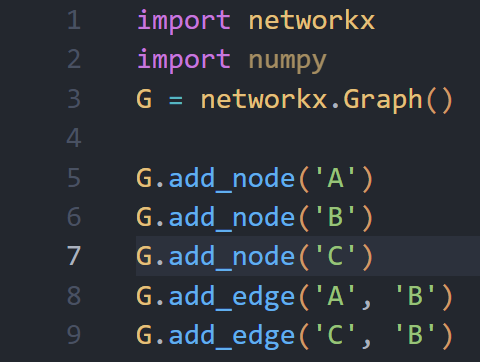
\includegraphics[width=8cm]{images/add_nodes_add_edges.png}\\
        The above code does the following: it imports the Networkx package for us to use, creates a 'graph' object called G, creates nodes A, B, C, then adds two edges between A and B and B and C.\\
        However that is too clunky for normal use so the Networkx package provides functions such as:
        \begin{verbatim}networkx.complete_graph(5)\end{verbatim}
        to generate a complete graph with 5 nodes in one line, but we still have the atomic control of the graph as in the first example.
        \subsection{Creating Random Graphs}
        To create a random graph on a piece of paper it is quite simple: Select $N$ nodes to add to the graph and $p$ probability, draw $N$ nodes on the paper, then go through every possible pair of nodes in the graph and draw an edge between them if when picking a random real number from [0,1] it is less than $p$. Networkx implements a function \verb|networkx.gnp_random_graph| to create a random graph using the following code:\\
        \begin{figure}[H]
            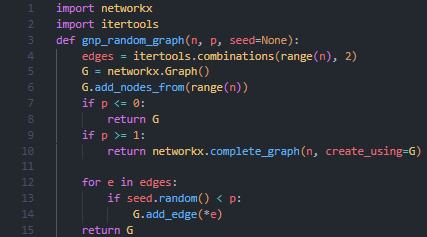
\includegraphics[width=8cm]{images/CreatingRandomGraphs.png}
            \caption{The Random Graph Function}
            \label{fig:RandomGraph1}
        \end{figure}
        Let's explain, the function takes $n$ (The total number of nodes) and $p$ (The probability of drawing an edge between a pair of nodes) as parameters. The \verb|itertools.combinations(range(n),2)| creates s list of every combination of 2 numbers up to $n$ i.e. (0,1), (0,2), (1,2) and so on, then to graph $G$ we add $n$ nodes, if $p = 0$ then there are 0 edges in the graph, so it stays empty and if $p =1$ then every node is attached to every other node, so it becomes a complete graph, if neither of those are true then we loop through all the possible combinations of nodes and choose a random number from $[0,1]$ and if that is less than $p$ we add an edge between those nodes.
        \subsection{Creating Barabasi-Albert Graphs}
        First let us describe how to create Barabasi-Albert Graphs on a piece of paper. To create a Barabasi-Albert Graph we must first start with a "seed" graph (An already drawn graph that we will grow using the Barabasi-Albert Model) then we will define two more parameters $n$ for the total number of nodes we want this new graph to have and $m$ the number of edges we will add each iteration of the model. The algorithm works in the following way: take your "seed" graph and assign each node on the graph a probability $p$ according to its degree $k$ using the formula $p(k_{i}) = \frac{k_{i}}{\sum_{j} {k_{j}}}$ we then randomly select $m$ unique nodes according to the probabilities calculated (this can be done by label each node 1 to n then write on a piece of paper that label for each node, then fold the paper a number of times proportional to its probability for example folding 0.2 twice but 0.2 five times then randomly choosing the papers), add 1 new node to the graph and draw an edge from this new node to each of the randomly preexisting nodes, repeat this until we have $n$ nodes on the graph.\\
        As Barabasi-Albert graphs are the main focus of this project we will now show how they are created in networkx. 
        \begin{figure}[H]
            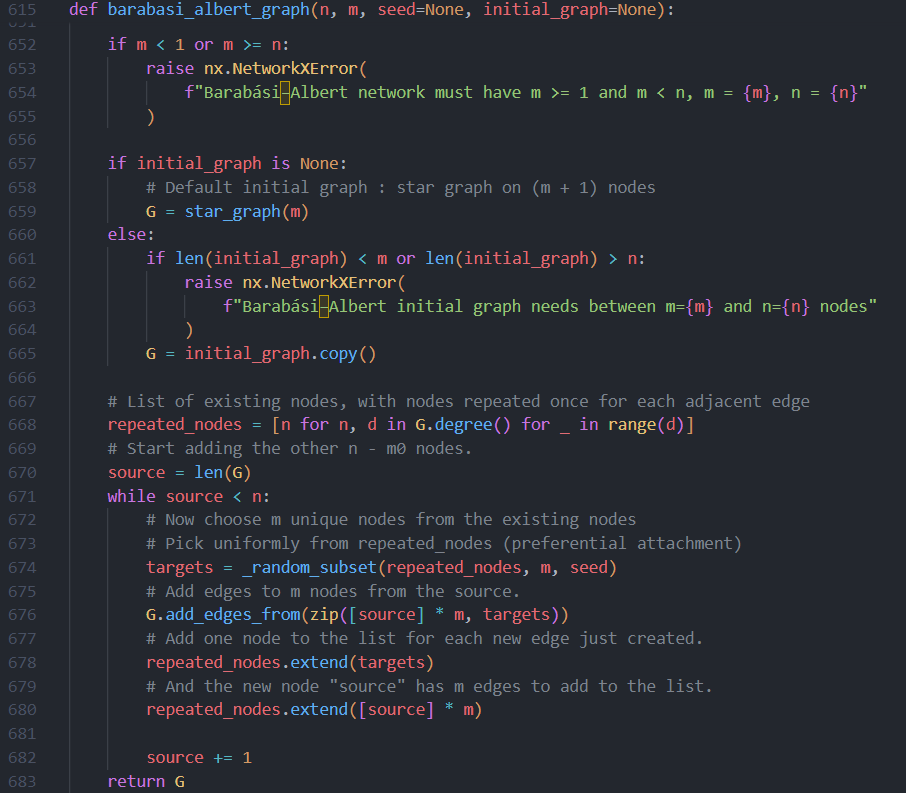
\includegraphics[width=8cm]{images/BARABASI_FUNC.png}
            \caption{The Barabasi-Albert Graph Function}
            \label{fig:Barabasi-Albert function1}
        \end{figure}
        This is the Barabási-Albert function from Networkx. It takes 4 parameters, $n$,$m$, \verb|seed|, and \verb|initial_graph|. $n$ and $m$ are simply the same as explained above, \verb|seed| is for the random functions later so we can control the behavior,  \verb|initial_graph| is where we input our 'seed graph' for the model to build on (If no graph is provided then it uses a Star graph with $(m+1)$ nodes). The function then creates a list of nodes: \verb|repeated_nodes| where each node is repeated equal to its degree (A node with degree $5$ is repeated 5 times) then takes random samples from this list to create the preferential attachment then finally returns the Barabási-Albert graph. 
        
        \subsection{Gaining Information From Graphs}
        Methods in networkx allow us to extract key information from the graph objects such as \verb|G.number_of_edges| which returns the number of edges that are contained in graph $G$ or \verb|networkx.all_neighbors(G,n)| which returns all the neighbors of node $n$ in graph $G$.
            
    
    
\printbibliography
\end{document}